%!TEX root = ../main.tex

\section{Pre-analysis} % (fold)
\label{sec:preanalysis}

For this semester we have chosen the theme \emph{Sonification}. 
Sonification is basically the use of non-speech audio to convey or perceptualize data~\cite*{Wiki2014-2}. 
In investigating sonification it is clear that there are more ways of sonifying data (see \enquote{Sonification Techniques} section~\ref{ssub:sonification_techniques}), depending on what kind of data is to be converted, and how that information is to be displayed and interacted with.
Sonification is used in various applications and projects (see \enquote{Examples of uses of sonification} in section~\ref{ssub:examples_of_sonification}), but sonification does face some challenges in its current state. 
The main problem is that it is difficult to provide adequate context for interpreting sonifications of data \cite*{Kramer1993}. 
To see to what extend this challenge can be overcome, first one must find data to be sonified.

One area which contains different sorts of data that theoretically could be sonified is weather data. 
Some of these could be: temperature (degrees), sunny or cloudy (either or), wind speed (meters per second), visibility, precipitation (rain/sleet/snow/hail measured in millimeters). 
These data have a different range of values. 
For instance, temperature could be an array of degrees and overcast can be a boolean value of yes or no. 
This means that theoretically a lot of different sonification techniques can be applied to this kind of information. 
Aside from being sonifiable, weather information is not usually presented as sound (see \enquote{Weather Data} section~\ref{sub:weather_data}), and could therefore possibly make for an interesting study and test of whether there could be advantages to combining non-speech audio with imagery, or possibly presenting the weather data as audio on its own, in addition to answering the question of to what extent it is possible to provide adequate context for interpreting the data.

We would like to investigate if visually presented weather data can actually be understood, and to which degree, if converted to non-speech sound using sonification. 
Can sonification of some of these data maybe even make the weather information more understandable or relatable? 
For instance, is information about wind or downpour more relatable as sound than numbers? 
These discussions have led us to the following Initial Problem Statement:

\subsection{Initial Problem Statement} % (fold)
\label{sub:initial_problem_statement}

\enquote{Is it possible to successfully use sonification to convey relevant information about weather conditions as efficiently as visually represented weather conditions/data?}

% subsection initial_problem_statement (end)


\subsection{Sonification} % (fold)
\label{sub:sonification}

Now that we have an idea of what kind of data we want to sonify, we will first look into the basics of sonification. 
What it is, and how it is used so we can begin to plan sonification of weather data, and the best approach/technique for doing this.


\subsubsection{What is Sonification?} % (fold)
\label{ssub:what_is_sonification_}

Sonification is used to convey information through non-speech audio, to get a better understanding of what that is; we will explain what kind of communication methods that are most common and examples of their functions.
These are visualization, auditory communication and sonification.
Sonification is a subcategory of audification, and visualization is the counterpart to audification and is also the most commonly used method for displaying weather data. 
Both of them can supplement each other~\cite[Ch. 1]{Hermann2011}.

Visualization is the communication method that we perceive through our eyes e.g. posters, TV, computer, traffic lights, chat systems, pictures, sign language, body language etc. 
As of now most applications that show weather data uses visualization methods, for instance, showing the temperature in numbers or a weather condition as an image~\cite[Sec. 1]{Friendly95}.

Auditory communication is data that we perceive through our ears like sonification, but unlike sonification, auditory communication can use speech, which occurs in for instance, radio, TV, computers, telephones, all kinds of equipment and applications that allow you talk with people over distance. 
Sonification only uses non-speech audio to convey information. 
An example is the traffic light junctions all around Denmark. When you near a crosswalk you will hear 2 different sounds. 
Both sounds are the same, but they consist of different paces of rhythm. 
One sound (slow) indicates it is a red light, while the other (fast) indicates it is safe to walk. 
This helps blind people know whether to cross or not, and is an example of sonification. Sonification is a subset of auditory displays. 
There are several uses of sonification, and these will be described in detail below.

% subsubsection what_is_sonification_ (end)


\subsubsection{Examples of uses of sonification} % (fold)
\label{ssub:examples_of_sonification}

Now that sonification has been defined, let us delve further into the topic and see what some of the uses for sonification could be. 
A good example to start out with is the use in the medical industry. 

From the beginning of medical school, students are taught to use stethoscopes to listen to tissue, gases and blood pumping through veins~\cite[Ch. 1]{Barrass1999}. 
Much of the data used for diagnosing a patient’s current status is shown in numbers or graphs, but a graph can be distracting during a demanding task, and it is possible to synthesise sounds to represent this data instead.
Medical students were shown to perform better in a setting where some dynamic variables about the patients status were presented with sounds rather than graphs~\cite[Ch. 1]{Barrass1999}. 
It is also used in MRI scans to identify unhealthy regions of the brain, and listening to such data might help a doctor diagnose an illness that otherwise goes undetected~\cite[Ch. 1]{Barrass1999}. 
There also exists multimedia programs that can make maps and text more accessible to visually impaired people.

Audiograf is an application that generates sound from part of a diagram selected with finger touch~\cite[Ch. 2]{Barrass1999}. 
Other programs exist such as Mercator, which makes it easier for a blind person to use graphical computer interfaces, by mapping navigation and buttons into auditory cues. 
Some web browsers have also been enhanced in a similar way, by using sonifications to present download times, layout, hyperlinks and more~\cite[Ch. 2]{Barrass1999}.

It is stated that gadgets and applications for the visually impaired using sonification have been mined thoroughly~\cite{Girvan2005}, but scientific alternatives also exist. 
An example of this is the ULTRA (Universal Laboratory Training and Research Aid), which is a device for blind science students created by David Lunney and Robert Morrison. 
ULTRA can be interfaced to give speech and present readouts from laboratory equipment such as pH probes and resistance thermometers~\cite{Girvan2005}.

There have also been attempts to create location devices as a replacement for guide dogs. 
For example, Dr. Leslie Kay’s \enquote{Sonic Torch}, a device using traditional sonar technology, which uses a bat-like frequency sweep to return detailed textural information~\cite{Girvan2005}.

\begin{figure}[!htbp]
    \centering
    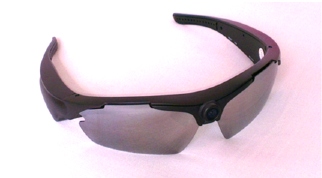
\includegraphics[width=0.7\textwidth]{images/Sonification1.png}
    \caption{Sonic Torch by Dr. Leslie Kay.}
    \label{fig:sonification1}
\end{figure}

Another attempt at a location device is created by Dr. Peter Meijer and is called vOICe. 
This works by taking the input from a digital camera, either a mounted one or the camera from a cellphone, and using software to sweep the image with a vertical scan line. 
It then sonifies features in the scan by representing vertical position as pitch, horizontal position as time, and brightness by increasing or decreasing volume~\cite{Girvan2005}. 
An interesting result that came from using this device was that a user reported experiences of seeing depth in different places throughout her house. 
On Dr. Meijer website \url{www.seeingwithsound.com}, a demo of vOICe made in Java can be found. 
On here the application is mentioned as \enquote{Augmented Reality for the Totally Blind}. 
The above image shows an example of how a vOICe device can look. 
The camera in the center is what captures the image then processed as previously mentioned.

As a last example regarding blind users, Joshua Miele of the Smith Kettlewell Eye Research Institute in San Francisco has written braille support for MATLAB and the sonification toolbox for blind engineers and scientists~\cite{Girvan2005}.

Generally, all these examples of technology tell us one thing. 
Technologies exist in the world where people have successfully used sonification to assist in everyday situations. 
The examples range from critical equipment dealing with life and death, to people just getting to experience what it is like to have some sort of vision. 
This tells us that sonification has a wide area of use, and focusing further on sonification techniques and how weather data is perceived and displayed will give us a good basis to work from.

There are different techniques for sonification of data. 
These will be discussed below.

% subsubsection examples_of_sonification (end)


\subsubsection{Sonification Techniques} % (fold)
\label{ssub:sonification_techniques}

The investigation of different sonification techniques will give us options and direction for when we later have to implement these techniques to sonify weather data for testing.

\paragraph{Techniques} % (fold)
\label{par:techniques} \hspace{0pt} \\
One way of defining sonifications is describing them according to their sonification techniques. Alberto de Campo, University for the Arts, Berlin, Germany, has made a \emph{sonification design map}~\cite[pp. 15]{Hermann2011}, which features three broad categorizations of sonification approaches.

\begin{enumerate}
    \item Event-based
    \item Model-based
    \item Continuous
\end{enumerate}

The appeal of de Campo’s approach is that it allows for blurry boundaries between the categories and offers guidance for choosing a sonification technique.

In the book, The Sonification Handbook, co-authors Michael Nees of Lafayette College, Easton, Pennsylvania, USA and Bruce N. Walker, Georgia Institute of Technology, Atlanta, USA, give a brief overview of the above techniques employed in sonification~\cite[pp. 16-17]{Hermann2011}:

\subparagraph{Interactivity:} % (fold)
\label{subp:interactivity}
One of the elements to consider when discussing sonification techniques is the interactivity available (or unavailable) to the user of an auditory display. 
Interactivity with auditory displays ranges from completely non-interactive to completely user initiated.
Non-interactive sonification is often referred to as \enquote{concert mode}. 
In instances where the user is able to change and/or choose parameters of the display, has been referred to as \enquote{query based} or \enquote{conservation mode}. User input may also be the driving factor of the presentation of the sound. \enquote{For most sonifications to be useful there must at least be some sort of interactivity, even if it is just play/pause or replay of a certain sound.} 
% subparagraph interactivity (end)

\subparagraph{Parameter mapping (event-based sonification):} % (fold)
\label{subp:parameter_mapping_event_based_sonification_}
\enquote{Parameter mapping represents changes in some data dimension with changes in an acoustic dimension to produce a sonification}. 
Sound has many changeable dimension such as frequency, amplitude, phase etc.
The dimensionality of these data must however be constrained such that a perceivable display is feasible. 
The data changes may be discrete or qualitative. 
For instance, and alarm may be triggered by a discrete on or off threshold, or parameter mapping can be a series of discrete data which makes it seem more continuous. 
These event-based techniques have a passive mode of interaction. 
Some event-based sonifications are brief and offer limited opportunity for user input.
% subparagraph parameter_mapping_event_based_sonification_ (end)

\subparagraph{Model-based sonification:} % (fold)
\label{subp:model_based_sonification_}
The model-based approach is different from the event-based approaches in that instead of mapping data parameters to sound parameters, the developer builds a virtual model whose sonic responses to user input is derived from data. 
A model is a virtual instrument with which the user can interact with. 
The user input drives the sonification. 
The user learns to understand the structure based on the sonic feedback of the user’s input.
These types of sonification usually involves large numbers of data points and and high data dimensionality.
% subparagraph model_based_sonification_ (end)

\subparagraph{Audification (continues sonification):} % (fold)
\label{subp:audification_continues_sonification_}
Audification is a direct form of sonification where waveforms of periodic data are directly translated into sound. For instance, a Geiger counter gives the user constant sonic feedback of the radiation level by translating data of radiation level into sound.
% subparagraph audification_continues_sonification_ (end)

These are the main methods of sonification, but the different techniques might not all apply to the kind of sonification required for converting weather data. 
The delimitation and choice of the sonification technique(s) most suited for our project will be discussed later (see Analysis chapter).

First we must investigate which weather data makes sense to sonify. 
This investigation will begin with looking at different weather forecast media, in order to see what different weather informations are considered to be more relevant to the general public, as it might not be relevant or necessary to cover every aspect of weather forecast information. 

% paragraph techniques (end)

% subsection sonification (end)

\subsection{Weather Data} % (fold)
\label{sub:weather_data}

Now that we have an overview of what sonification is and some methods of application, we will begin to investigate what weather information is and what types of weather information is usually decided by different sources as being more relevant to the user. 
Gathering this knowledge of popularly presented weather information will help decide which weather information is most relevant for us to sonify in order to answer the question of how far it is possible to provide adequate context for interpreting sonifications of data.


\subsubsection{What is weather Data?} % (fold)
\label{ssub:what_is_weather_data_}
First off, what is meant by weather data? Weather data is derived from weather forecasting. 
Weather forecasting attempts to predict the state of the atmosphere for a given location, using science and technology.

\begin{quote}
``Weather forecasts are made by collecting quantitative data about the current state of the atmosphere on a given place and using scientific understanding of atmospheric processes to project how the atmosphere will evolve on that place.'' \cite*{Wiki2014-1}
\end{quote}

Weather forecasts are used for a variety of different purposes. 
For instance, weather warnings used to alert societies of dangerous weather, precipitation and temperature is important in agriculture, road surface conditions is important to traffic etc. 
On everyday basis, weather forecasts are used to determine what clothes to wear, traffic and travel time, and to plan outdoor activities on a given day.
Nowadays weather forecasting relies on computer-based models that take many different atmospheric factors into account~\cite{Shuman1978}.
There is a big range of different weather data, some of these are:

\begin{itemize}
     \item \textbf{Temperature/Dewpoint} - Current air temperature 2 meters above terrain.
     \item \textbf{Wind speed} - Average wind speed over 10 minutes, 10 meters above terrain.
     \item \textbf{Wind direction} - Average wind direction in degrees.
     \item \textbf{Air pressure} - Pressure at sea level measured i hPa (Hectopascal).
     \item \textbf{Humidity} - Current relative humidity measured 2 meters above terrain, measured in percent.
     \item \textbf{Precipitation} - Rain/sleet/snow/hail over the past ten minutes measured in mm.
     \item \textbf{Sun hours} - Hours with sun in a day.
     \item \textbf{Pollen Forecast} - The potency of the pollen. 
     \item \textbf{Sunrise / sunset} - Time of day where the sun rises and sets.
     \item \textbf{Cloud cover}
     \item \textbf{Wind chill} - The winds effect on air temperature.
     \item \textbf{Visibility} - How far can you see with clear line of sight.
     \item \textbf{UV-index} - Intensity of UV radiation.
     \item \textbf{Fronts} 
     \item \textbf{Source Regions} - Where the air is coming from.
     \item \textbf{Drought} - Risk of drought. Presented as a scale.
 \end{itemize}

These are just some of the weather data available in modern weather forecasting. 
Not all of these are necessarily relevant to one single individual, and weather forecasts meant for the general public (not fields of work/study that require very specific weather data) limit the amount and range of weather data presented for the sake of clarity and time (both to present the information but also the time required by the individual to get the information relevant to most). 
Below are some examples of what types of weather data have been chosen to be presented to the viewer on certain weather websites and popularly used weather applications. 
This weather information will later in the report be delimitated for testing purposes of the challenge of providing adequate context for interpreting sonifications of the weather data.

% subsubsection what_is_weather_data_ (end)

\FloatBarrier
\subsubsection*{DMI.dk (Danish Meteorological Institute)} % (fold)
\label{ssub:dmi_dk_danish_meteorological_institute_}

DMI.dk is the website of the danish national meteorological institute. 
It is arguably the most well known website containing weather information, in Denmark. 
The website contains a huge amount of weather data, which makes it a bit difficult to navigate and find even the basic weather forecast of the day/week. 
Navigating through the site you will however be able to find information about the atmosphere in a given region such as:
radar images of precipitation, satellite images, lightning probability, ozone measurements, snow depths, and drought indexes, in addition to the more standard weather information such as wind speed, temperature, precipitation (represented as a graph) and so on. 

\begin{figure}[!htbp]
     \centering
     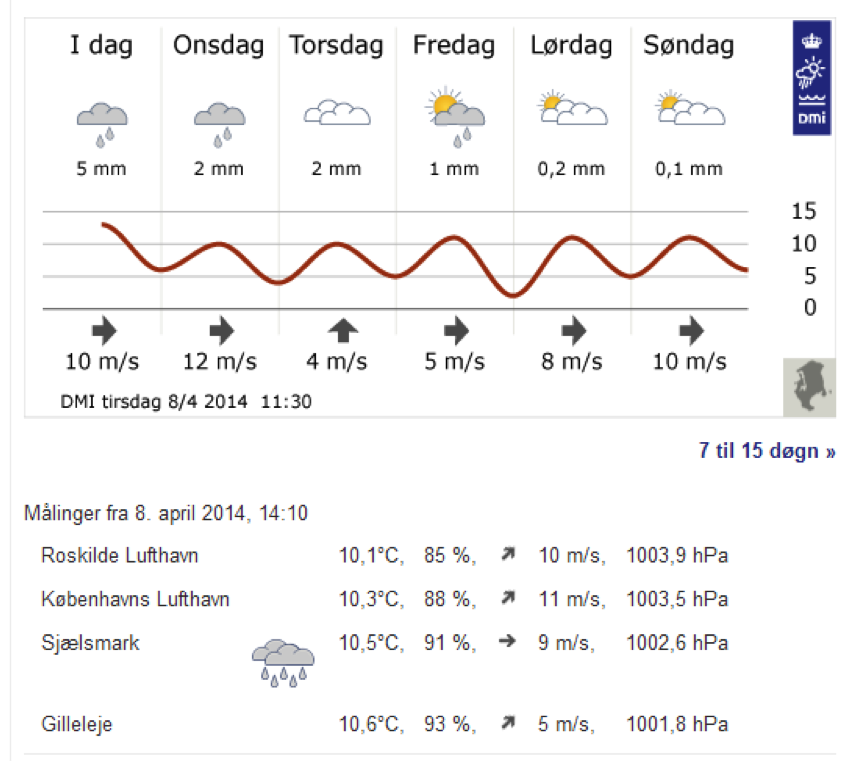
\includegraphics[width=.75\textwidth]{images/Dmi1.png}
     \caption{7-day forecast from DMI.dk}
     \label{fig:dmi1}
 \end{figure}

However, in order to give a shorter, but more clear forecast, you have the option to get a graphically presented 7-day prognosis (Figure~\ref{fig:dmi1}).


This is the basic weather data chosen to be relevant to the general public, and thus this is the prognosis we will be comparing with the other forecasts. 
The 7-day prognosis on DMI.dk contains information about:

\begin{itemize}
    \item Precipitation
    \item Cloud cover
    \item Temperature
    \item Wind speed
    \item Wind direction
\end{itemize}

Additionally, information measured at a certain point of the current day at predetermined locations (April 8, 2014 - 14:10) is presented:

\begin{itemize}
    \item Temperature
    \item Visibility
    \item Wind direction
    \item Wind speed
    \item Atmospheric pressure
\end{itemize}

There is also a summary of the current day’s forecast.

% subsubsection dmi_dk_danish_meteorological_institute_ (end)

\FloatBarrier
\subsubsection*{TV2 Vejret App} % (fold)
\label{ssub:tv2_vejret_app}

TV2 Vejret is a weather app developed by danish TV channel TV2 for iOS and Android. 
The app pulls weather data directly from the TV2 weather center, where the TV stations meteorologists work on predicting the weather for the TV2 news, website and the weather app.


The app finds the phones current location via GPS and retrieves weather information about that area. 
In terms of relevant data, the app gives a fairly limited amount of information (at least compared to DMI.dk), but covers the basic data such as:

\begin{itemize}
    \item Precipitation
    \item Wind speed
    \item Wind direction
    \item Sun up/down
    \item UV index
    \item Cloud cover
    \item Temperature
\end{itemize} 

From figure~\ref{fig:tv21} it is apparent that most of the information is only presented for the current time of day. 
Prognosis for the next 14 days is limited to:

\begin{itemize}
    \item Cloud cover
    \item Temperature
    \item Precipitation
    \item Wind speed
    \item Wind direction
\end{itemize}

\begin{figure}[!htbp]
    \centering
    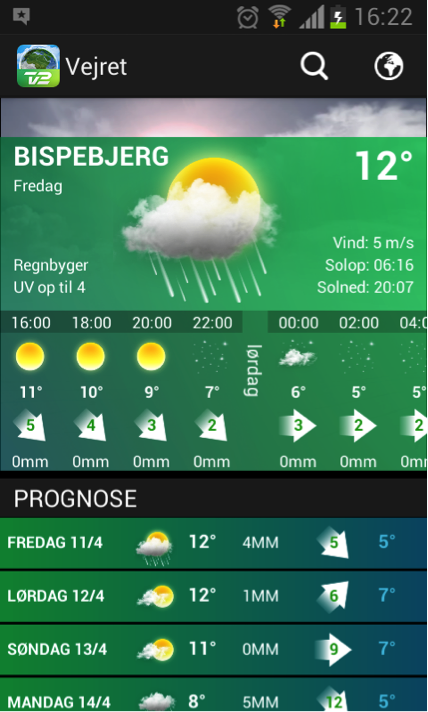
\includegraphics[width=.4\textwidth]{images/Tv21.png}
    \caption{TV2 weather app}
    \label{fig:tv21}
\end{figure}

The app does not however provide radar, heat maps or other more advanced features. 
It has the typical amount of information about the weather for an app, but where the app sets itself apart from the competition, is due to the fact that it is a TV-channel app. 
This means that the app contains video streams of the latest weather forecasts from TV, and other weather related news. 
This can be useful if you want a more detailed forecast with certain highlights about the current and forthcoming weather. 

% subsubsection tv2_vejret_app (end)

\FloatBarrier
\subsubsection*{Yahoo Weather} % (fold)
\label{ssub:yahoo_weather}

Yahoo Weather is an app for iOS and Android which shows the weather in your current location, or if you want, in other locations around the world as well. 
The app contains a lot of the same information that other weather applications do, it is the design of the interface and layout which sets it apart from other apps. 
The application has received the \enquote*{'Apple Design Award'} because of it's aesthetics. 
One of the features of the design, which has gotten a lot of praise, is that the app finds beautiful images of your location on Flickr (an online image database), taking into account the time of the day and current weather condition, of your location and the photos, and uses these as the background of the weather information. 
Aside from this unique approach to visually presenting you surroundings, the interface itself was also very well received by critics. 


In addition to having a very manageable interface, the app actually also contains a great deal of detailed weather information. This data includes:

\begin{itemize}
    \item Temperature
    \item Cloud cover
    \item Precipitation
    \item Probability of downpour (percentage)
    \item Wind Speed
    \item Wind direction
    \item Pressure
    \item Chill factor
    \item Humidity
    \item Visibility
    \item UV-index
    \item Sunrise/sunset
    \item Moon position
    \item Heat map
    \item Wind map
    \item Satellite map
\end{itemize}

Again, as with the TV2 Vejret app, most of the detailed information is only available for the current time on the current day. 
For the 5 and 10 day forecasts there is only information about:

\begin{itemize}
    \item Cloud cover
    \item Day/night temperature peaks
\end{itemize}

Because of the apps very minimalistic design approach the screen is not overloaded with all sorts of data about the weather.
It uses subtle animations eg. a windmill spinning at a rate according to the current wind speed to illustrate more palpable information about the wind speed. 
Another way the application tries to present information relevant to the user, is by adding customization. 
The user can drag the different modules around to bring the most viewed ones to the top of the screen, limiting the amount of scrolling around to get information you want.

\begin{figure}[!htbp]
    \centering
    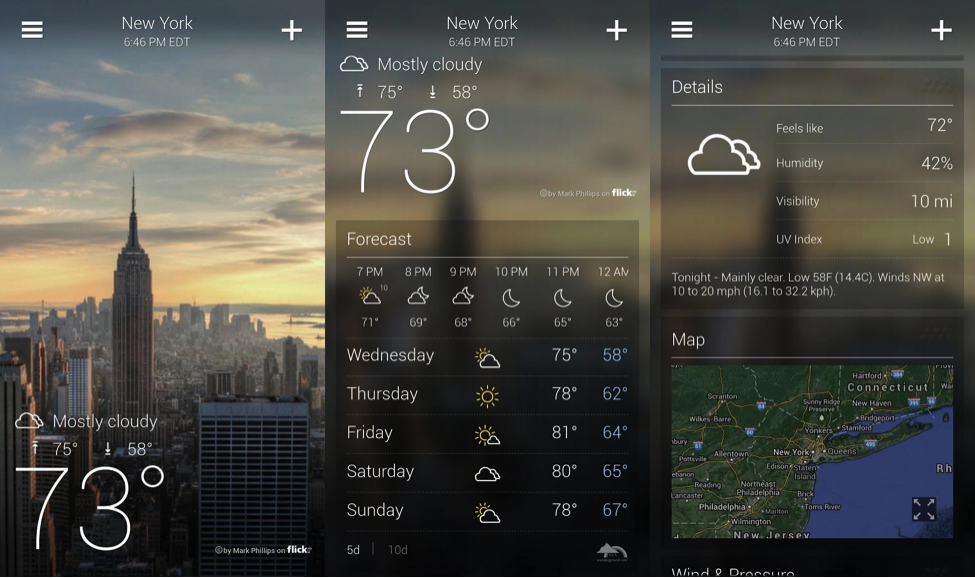
\includegraphics[width=0.95\textwidth]{images/Yahoo1.png}
    \caption{Yahoo weater app}
    \label{fig:yahoo1}
\end{figure}

So all in all, the app does contain a lot of information about the weather, and instead of the developers delimitating the information and deciding which weather data i relevant to the user, they allow the user the option of customizing the app, deciding themselves what information is relevant. 

% subsubsection yahoo_weather (end)

\FloatBarrier
\subsubsection*{InstaWeather} % (fold)
\label{ssub:instaweather}

InstaWeather is a weather application that focuses a lot on being a visual application. 
The amount of information about the weather depends on which skin to the application that you want to use. 
The information given can be limited to only being the temperature, a symbol that shows the weather condition and a small forecast. 
Some skins can also be very detailed and give information air pressure, temperature, rain, wind power and direction. 
The app is very customizable so you can change pictures so it feels more personal. 
The main feature in this application is that it borrows the picture sharing ability from Instagram. 
This means that the user can take a picture and send it to a friend with weather information added to the picture.  

\begin{figure}[!htbp]
    \centering
    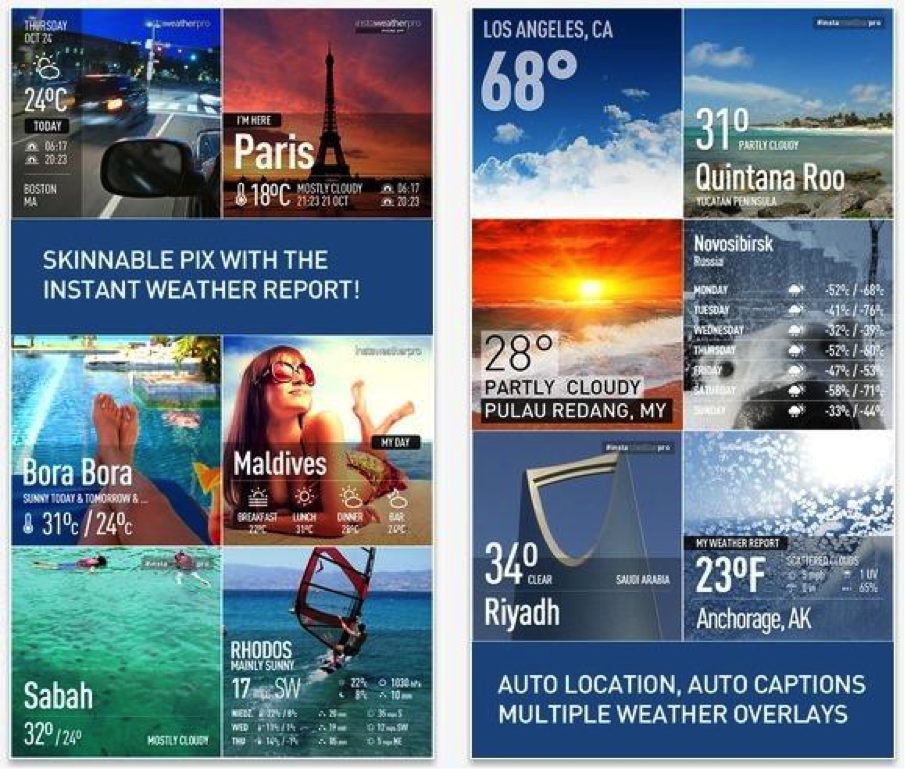
\includegraphics[width=.7\textwidth]{images/Instaweather1.png}
    \caption{InstaWeather}
    \label{fig:instaweather1}
\end{figure}

It is difficult to write about what relevant weather information is in regards to this application, because the user wholly decides for him/her self, what that is. 
It is in some way the most relevant weather information can be to a specific user, if that person puts in the time to customize the application for his or her needs. 
It does not however tell us much about what is in general considered to be chosen as relevant weather data.

% subsubsection instaweather (end)

Which weather information to be sonified for our test will be decided later in the Design chapter through user testing.

% subsection weather_data (end)


\subsection{Final Problem Statement} % (fold)
\label{sub:final_problem_statement}

Now that we have an idea of the process of sonification, and having revised typical visually presented weather forecasts and their content, we have to find out whether it is possible to provide adequate context for interpretation of weather data with the use of sonification. 
This will be investigated by comparing to visual data presentation in order to see to what extent it is possible to provide an understanding of these data as non-speech audio. This brings us to the final problem statement:

\enquote{To what extent is it possible to convey weather information, solely as a nonspeech auditory display, using sonification techniques, and be as intuitively understandable as visually presented weather information, where intuitive is defined as knowing by intuition?}

% subsection final_problem_statement (end)

% section preanalysis (end)
